\chapter{Evidencia de funcionamiento}\label{chap:performanceEvidence}

En este capítulo se comparan los cálculos de la librería \Materia con aquellos en la literatura.  Se reproducen algunas figuras del libro 'Modeling Vapor-Liquid Phase Equilibria'\cite{mvle}.

En este capítulo mostraremos una figura por regla de mezclado ó por modelo de actividad. En la página de internet \url{http://chimicae-materia.rhcloud.com/} se pueden encontrar un mayor número de figuras.

La primera comparación, ver figura \ref{fig:mpvdw}, se realiza para el sistema (1)Metano,(2)Pentano con la regla de mezclado de Van Der Waals y la ecuación de estado cúbica PRSK a las temperaturas de $310, 377, 444  [K]$ con el parámetro de interacción $k12=0.0215$. Podemos observar que el diagrama generado con la librería \Materia (Diagrama izquierdo de la figura \ref{fig:mpvdw}) es muy semejante al de la literatura (Diagrama derecho de la figura \ref{fig:mpvdw}).

\begin{figure}[H]
	\begin{tabular}{c c}
		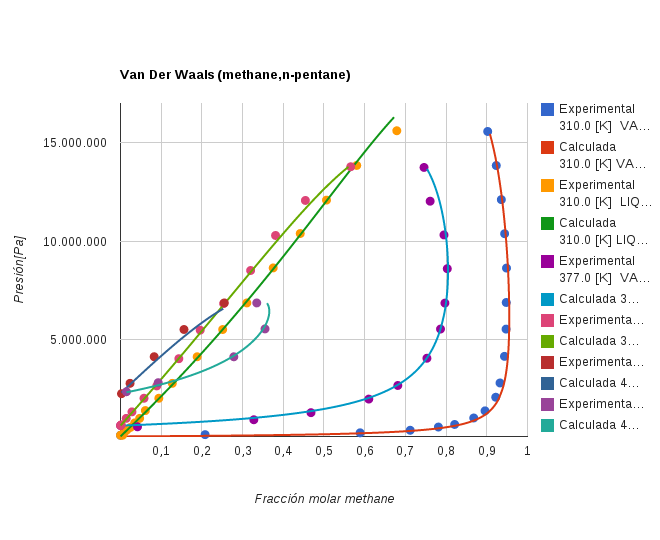
\includegraphics[scale=0.44]{vdwmpMateria.png}
		&
		 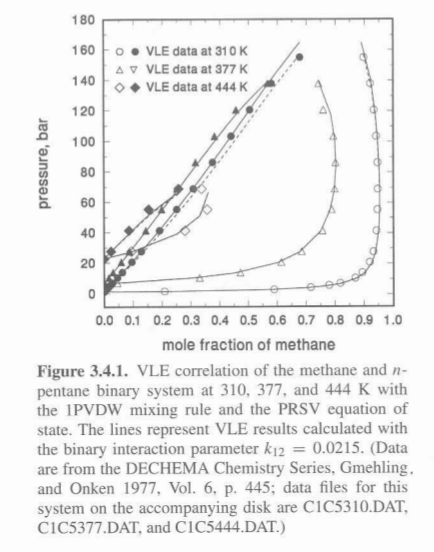
\includegraphics[scale=0.44]{mpvdw.png}
	\end{tabular}
	\caption{Comparación para el sistema (1)Metano,(2)Pentano con la regla de mezclado de Van Der Waals y la ecuación de estado PRSK. Izquiera figura obtenida con la librería \Materia, Derecha Figura del libro \cite{mvle} página 27.} 
	\label{fig:mpvdw}
\end{figure}

Para la regla de Van Der Waals de dos parámetros '2PVDW' se muestra el sistema (1)2-Propanol,(2)Agua a la temperatura $353[K]$ con los parámetros binarios $k12/k21 = 0.0953/0.0249$, ver la figura \ref{fig:pw2pvdw}. Solo se reproduce la línea sólida de la figura del libro, que representa el modelo de dos parámetros.

\begin{figure}[H]
	\begin{tabular}{c c}
		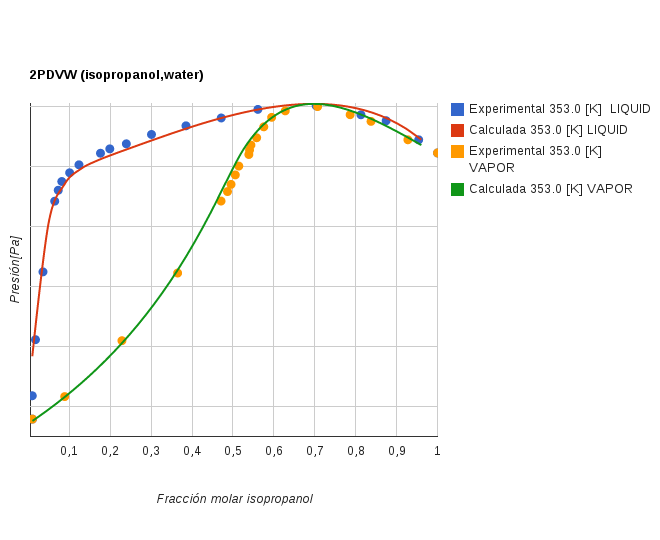
\includegraphics[scale=0.44]{pw2pvdwMateria.png}
		&
		 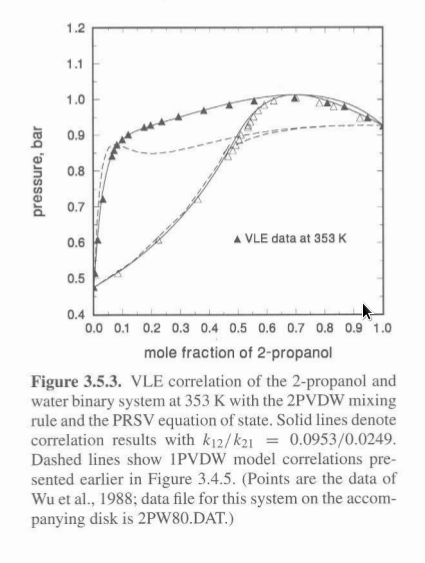
\includegraphics[scale=0.44]{2pvdw2propanolwater.png}
	\end{tabular}
	\caption{Comparación para el sistema (1)2-Propanol,(2)Agua con la regla de mezclado de Van Der Waals de 2 parámetros '2PVDW' y la ecuación de estado PRSK.  Izquiera figura obtenida con la librería \Materia, Derecha Figura del libro \cite{mvle} página 37.} 
	\label{fig:pw2pvdw}
\end{figure}

Para la regla de mezclado de Huron Vidal Original 'HVO' se eligió el sistema (1)Dióxido de carbono,(2)Propano a las temperaturas de $277, 310, 344 [K]$ con el modelo de actividad de Van Laar y los parámetros binarios $\Lambda_{12}/\Lambda_{21}=1.1816/1.6901$, ver la figura \ref{fig:cdhvvl}. Solo se reproducen las líneas discontínuas de la figura del libro que representan al modelo de Huron y Vidal.

\begin{figure}[H]
	\begin{tabular}{c c}
		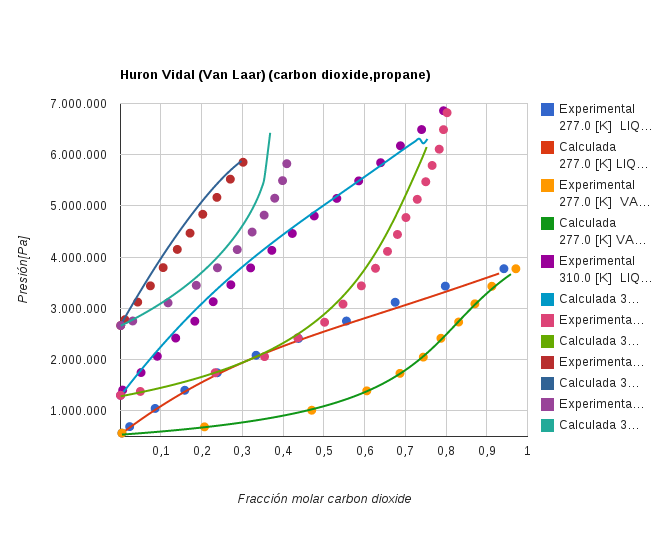
\includegraphics[scale=0.44]{cdhvvlMateria.png}
		&
		 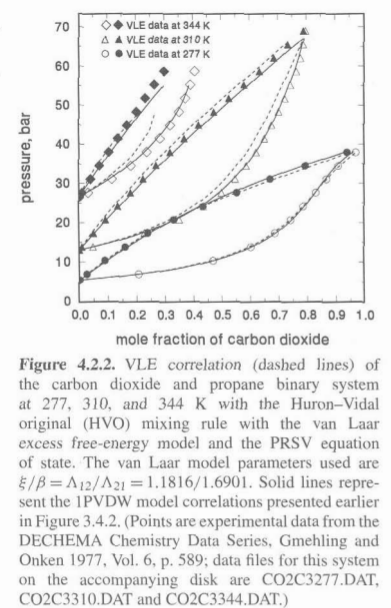
\includegraphics[scale=0.44]{cdhvvl.png}
	\end{tabular}
	\caption{Comparación para el sistema (1)Dióxido de carbono ,(2)Propano con la regla de mezclado de Huron y Vidal Original 'HVO' y el modelo de actividad de Van Laar y la ecuación de estado PRSK.  Izquiera figura obtenida con la librería \Materia, Derecha Figura del libro \cite{mvle} página 57.} 
	\label{fig:cdhvvl}
\end{figure}

La regla de mezclado de Huron Vidal Original 'HVO' y el modelo de actividad NRTL se comparó empleando el sistema (1)2-Propanol ,(2)Agua a la temperatura de $523 [K]$ con los parámetros binarios $\tau_{12} /\tau_{21}=0.392/4.1518$ y el parámetro $\alpha = 0.2893$, ver la figura \ref{fig:pwhvnrtl}. Solo se reproducen las líneas discontínuas de la figura del libro que representan al modelo de Huron y Vidal con el modelo de actividad de NRTL.
\begin{figure}[H]
	\begin{tabular}{c c}
		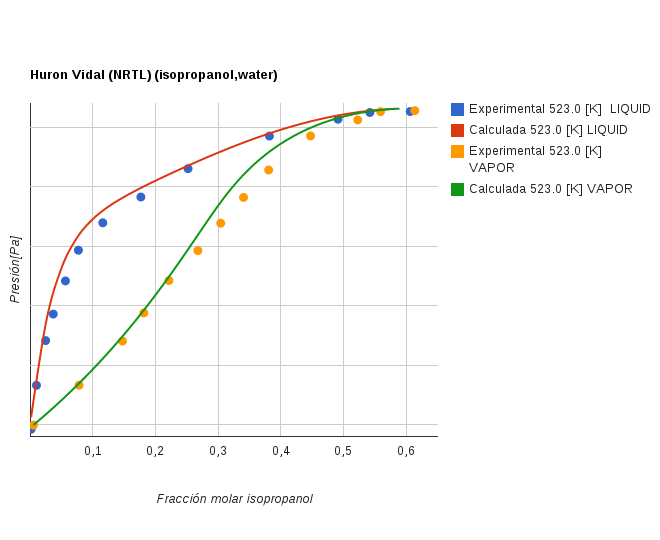
\includegraphics[scale=0.44]{pwhvnrtlMateria.png}
		&
		 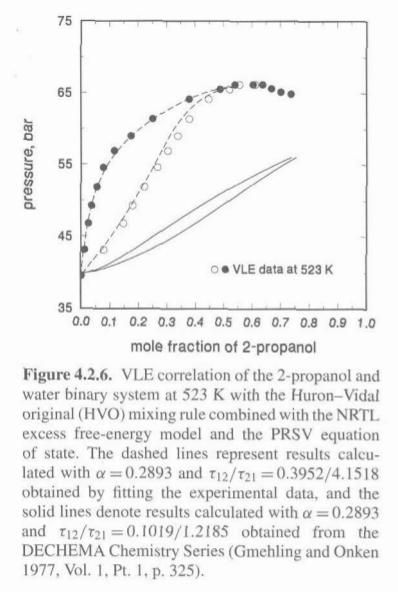
\includegraphics[scale=0.44]{pwhvnrtl.png}
	\end{tabular}
	\caption{Comparación para el sistema (1)2-Propanol ,(2)Agua con la regla de mezclado de Huron y Vidal Original 'HVO' y el modelo de actividad de NRTL y la ecuación de estado PRSK.  Izquiera figura obtenida con la librería \Materia, Derecha Figura del libro \cite{mvle} página 54.} 
	\label{fig:pwhvnrtl}
\end{figure}


La regla de mezclado de Wong Sandler 'WS' y el modelo de actividad UNIQUAC se comparó empleando el sistema (1)2-Propanol ,(2)Agua a la temperatura de $298 [K]$ con los parámetros binarios $\Delta u_{12} /\Delta u_{21}=837.65/-28.38$ y el parámetro $k12 = 0.15$, ver la figura \ref{fig:pwwsuniquac}. Solo se reproduce la línea continua de la figura del libro que representan al modelo de WS con el modelo de actividad de UNIQUAC.
\begin{figure}[H]
	\begin{tabular}{c c}
		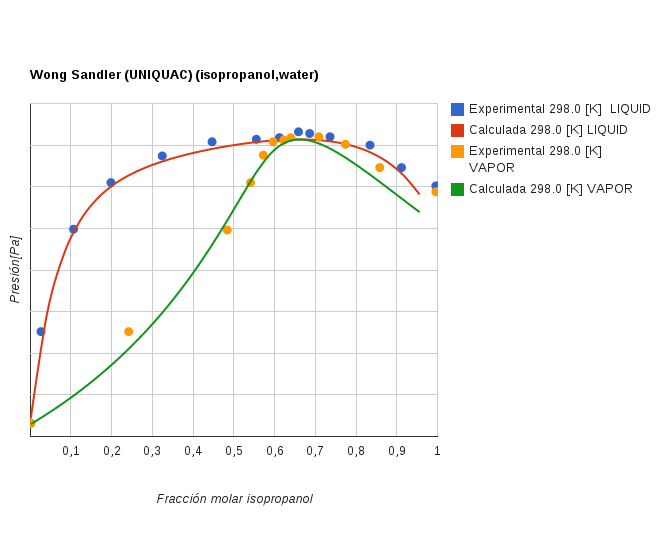
\includegraphics[scale=0.44]{pwwsuniquacMateria.png}
		&
		 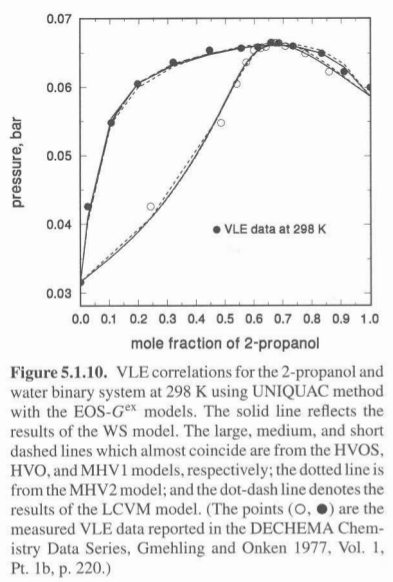
\includegraphics[scale=0.44]{pwwsuniquac.png}
	\end{tabular}
	\caption{Comparación para el sistema (1)2-Propanol ,(2)Agua con la regla de mezclado de Wong Sandler 'WS', el modelo de actividad de 'UNIQUAC' y la ecuación de estado PRSK.  Izquiera figura obtenida con la librería \Materia, Derecha Figura del libro \cite{mvle} página 85.} 
	\label{fig:pwwsuniquac}
\end{figure}

Con las figuras presentadas en este capítulo se demuestra la semejanza de los cálculos de la librería \Materia con la literatura. Los ligeros cambios pueden depender de las constantes de las expresiones de $\alpha$ para los compuestos puros, las propiedades críticas de los compuesots puros y la estabilidad de los métodos numéricos.